\newpage
\section{ERD}
\subsection{Diagram ERD}
\begin{figure}
	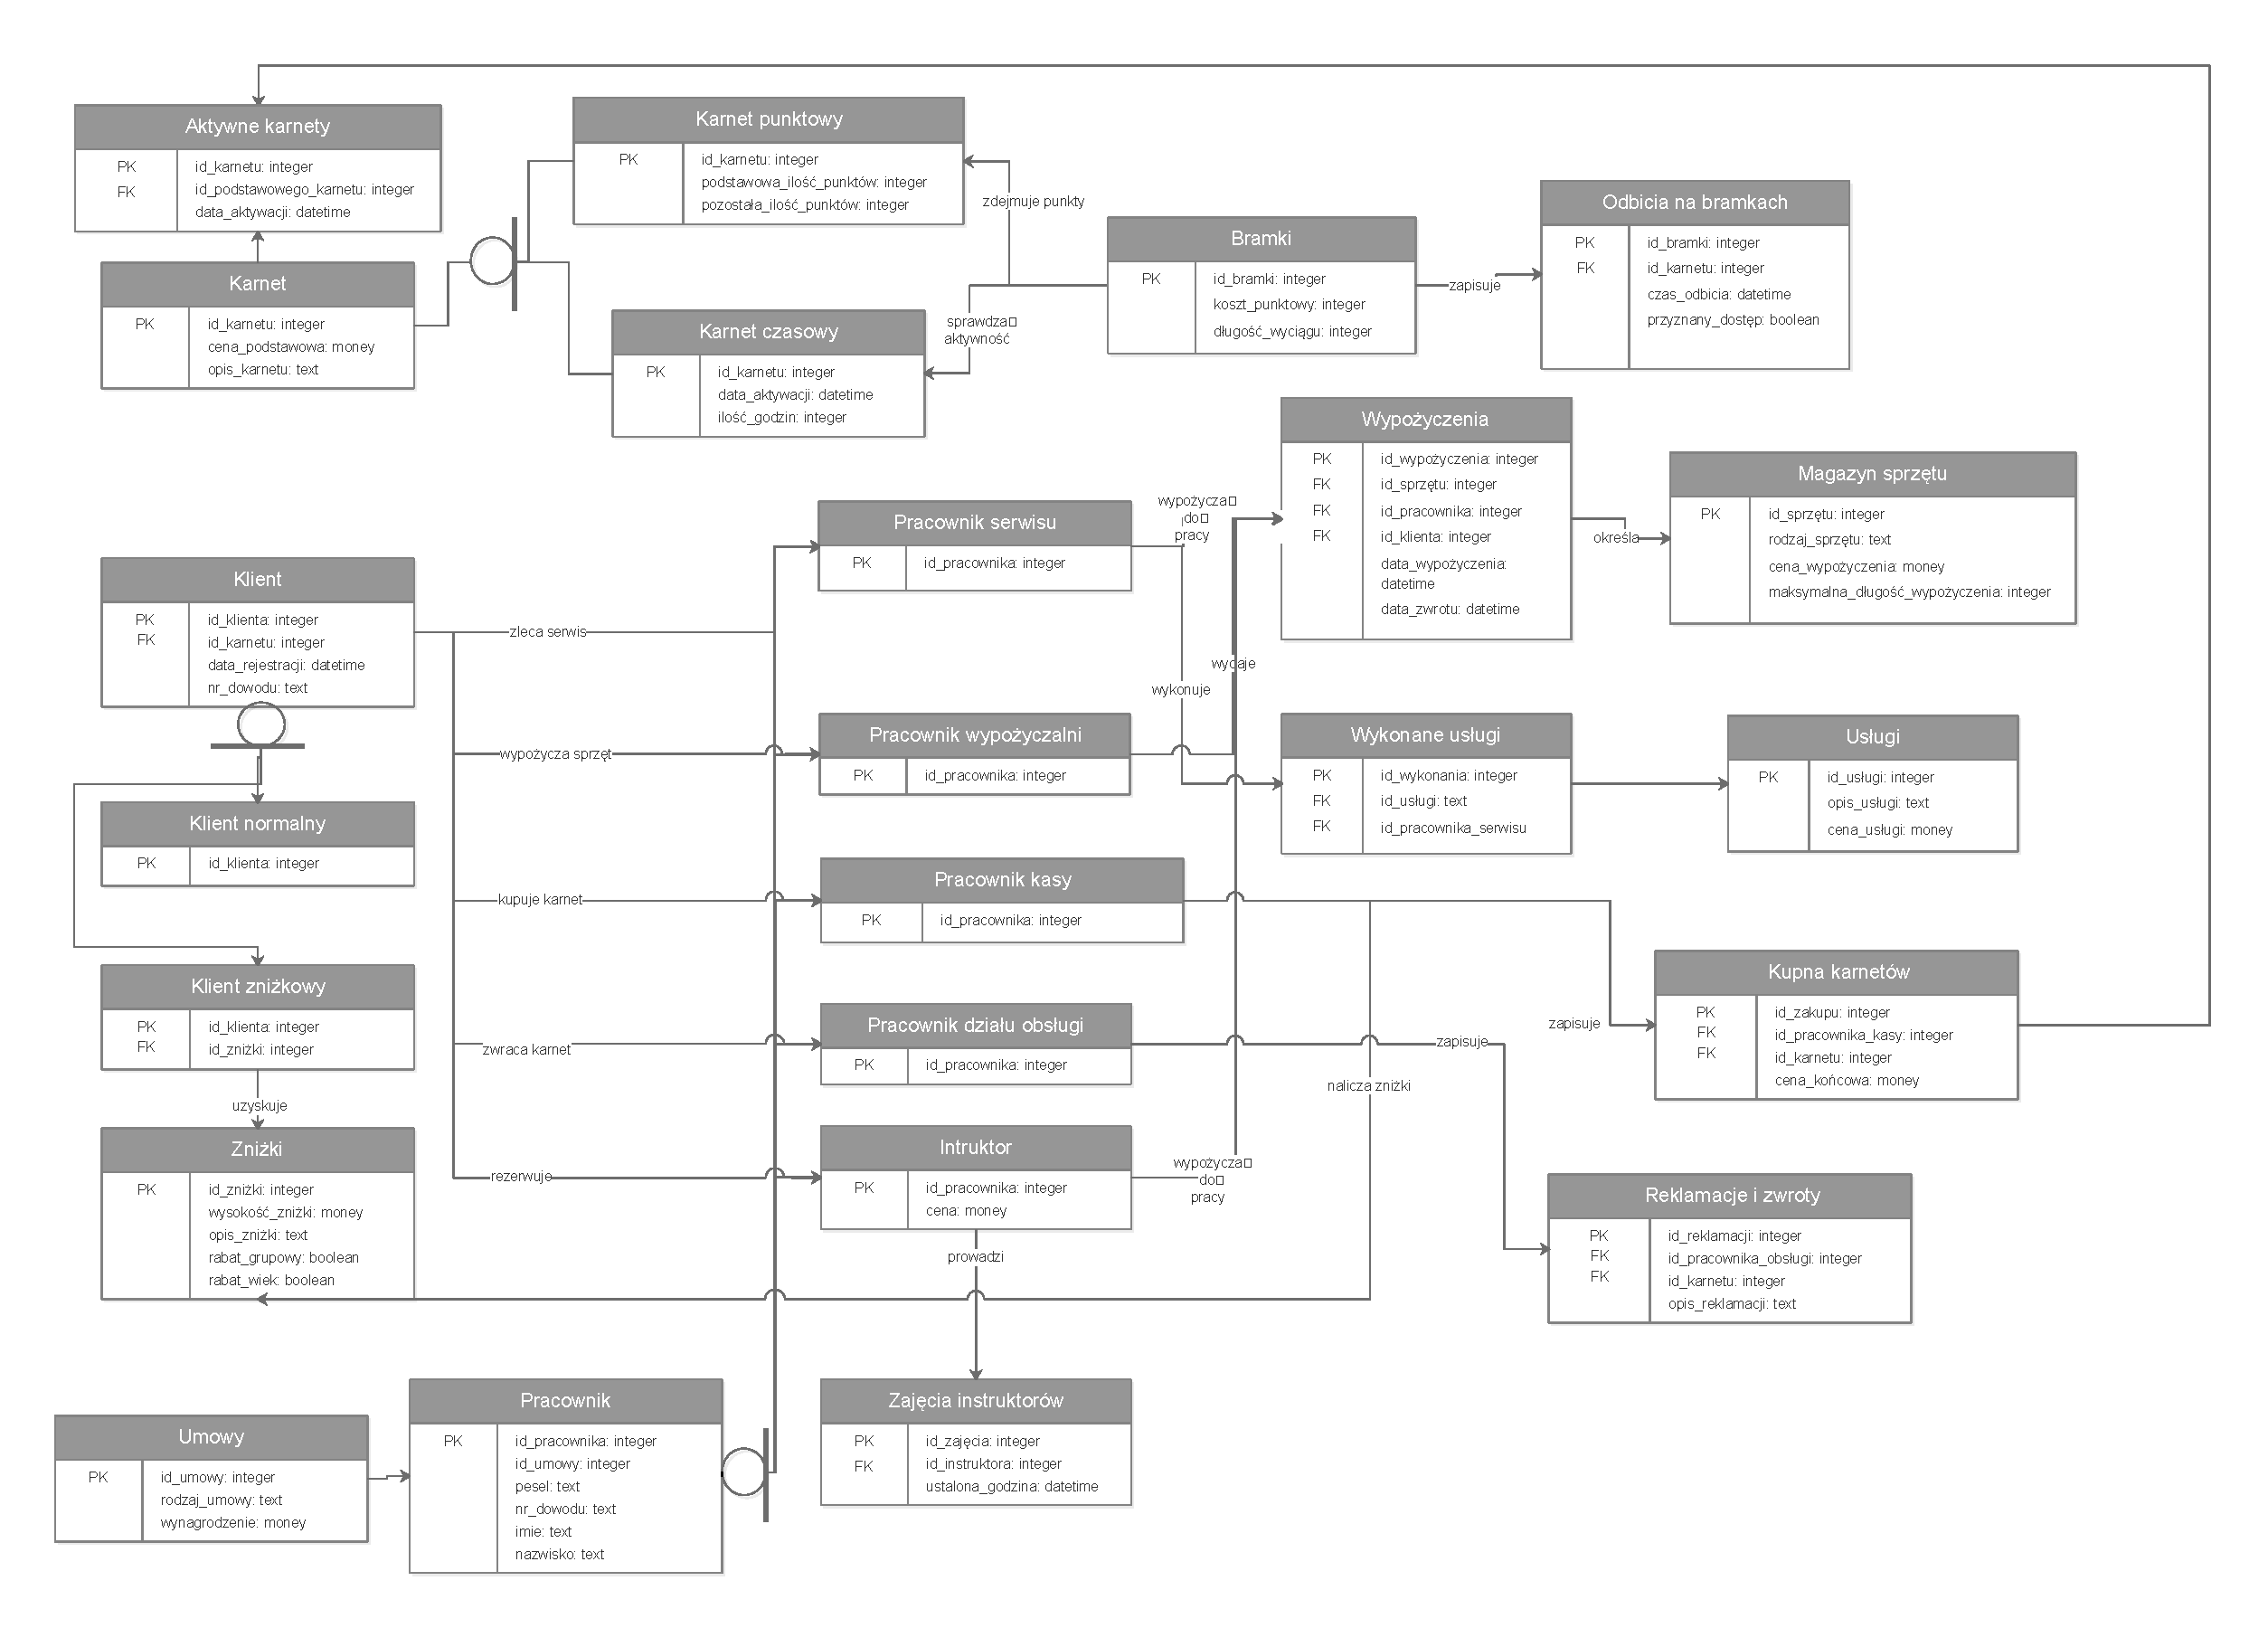
\includepdf[]{erd/erd}
\end{figure}

\newpage
\subsection{Klienci - opis}
\subsubsection{Klient}
\begin{table}[H]
	\centering
	\begin{tabular}{|c|c|c|c|}
		\hline
		Klucz & Nazwa atrybutu    & Typ danych & Obowiązkowy? \\ \hline
		PK    & id\_klienta       & integer    & tak           \\ \hline
		FK    & id\_karnetu       & integer    & nie           \\ \hline
		      & data\_rejestracji & datetime   & nie           \\ \hline
		      & nr\_dowodu        & text       & tak           \\ \hline
	\end{tabular}
	\caption{Klienci}
\end{table}

\subsubsection{Klient normalny}
\begin{table}[H]
	\centering
	\begin{tabular}{|c|c|c|c|}
		\hline
		Klucz & Nazwa atrybutu & Typ danych & Obowiązkowy? \\ \hline
		PK    & id\_klienta    & integer    & tak           \\ \hline
	\end{tabular}
	\caption{Klienci normalny}
\end{table}

\subsubsection{Klient zniżkowy}
\begin{table}[H]
	\centering
	\begin{tabular}{|c|c|c|c|}
		\hline
		Klucz & Nazwa atrybutu & Typ danych & Obowiązkowy? \\ \hline
		PK    & id\_klienta    & integer    & tak           \\ \hline
		FK    & id\_zniżki    & integer    & tak           \\ \hline
	\end{tabular}
	\caption{Klienci zniżkowy}
\end{table}

\subsection{Zniżki - opis}
\begin{table}[H]
	\centering
	\begin{tabular}{|c|c|c|c|}
		\hline
		Klucz & Nazwa atrybutu      & Typ danych & Obowiązkowy? \\ \hline
		PK    & id\_zniżki         & integer    & tak           \\ \hline
		      & wysokość\_zniżki & money      & tak           \\ \hline
		      & opis\_zniżki       & text       & tak           \\ \hline
		      & rabat\_grupowy      & boolean    & nie           \\ \hline
		      & rabat\_wiek         & boolean    & nie           \\ \hline
	\end{tabular}
	\caption{Zniżki}
\end{table}

\subsection{Pracownicy - opis}
\subsubsection{Pracownik}
\begin{table}[H]
	\centering
	\begin{tabular}{|c|c|c|c|}
		\hline
		Klucz & Nazwa atrybutu & Typ danych & Obowiązkowy? \\ \hline
		PK    & id\_pracownika & integer    & tak           \\ \hline
		FK    & id\_umowy      & integer    & tak           \\ \hline
		      & pesel          & text       & tak           \\ \hline
		      & nr\_dowodu     & text       & tak           \\ \hline
		      & imie           & text       & tak           \\ \hline
		      & nazwisko       & text       & tak           \\ \hline
	\end{tabular}
	\caption{Pracownicy}
\end{table}

\subsubsection{Pracownik serwisu}
\begin{table}[H]
	\centering
	\begin{tabular}{|c|c|c|c|}
		\hline
		Klucz & Nazwa atrybutu & Typ danych & Obowiązkowy? \\ \hline
		PK    & id\_pracownika & integer    & tak           \\ \hline
	\end{tabular}
	\caption{Pracownik serwisu}
\end{table}

\subsubsection{Pracownik wypożyczalni}
\begin{table}[H]
	\centering
	\begin{tabular}{|c|c|c|c|}
		\hline
		Klucz & Nazwa atrybutu & Typ danych & Obowiązkowy? \\ \hline
		PK    & id\_pracownika & integer    & tak           \\ \hline
	\end{tabular}
	\caption{Pracownik wypożyczalni}
\end{table}

\subsubsection{Pracownik kasy}
\begin{table}[H]
	\centering
	\begin{tabular}{|c|c|c|c|}
		\hline
		Klucz & Nazwa atrybutu & Typ danych & Obowiązkowy? \\ \hline
		PK    & id\_pracownika & integer    & tak           \\ \hline
	\end{tabular}
	\caption{Pracownik kasy}
\end{table}

\subsubsection{Pracownik działu obsługi}
\begin{table}[H]
	\centering
	\begin{tabular}{|c|c|c|c|}
		\hline
		Klucz & Nazwa atrybutu & Typ danych & Obowiązkowy? \\ \hline
		PK    & id\_pracownika & integer    & tak           \\ \hline
	\end{tabular}
	\caption{Pracownik działu obsługi}
\end{table}

\subsection{Instruktorzy - opis}
\subsubsection{Instruktor}
\begin{table}[H]
	\centering
	\begin{tabular}{|c|c|c|c|}
		\hline
		Klucz & Nazwa atrybutu & Typ danych & Obowiązkowy? \\ \hline
		PK    & id\_pracownika & integer    & tak           \\ \hline
		      & cena           & money      & tak           \\ \hline
	\end{tabular}
	\caption{Instruktor}
\end{table}

\subsubsection{Zajęcia instruktorów}
\begin{table}[H]
	\centering
	\begin{tabular}{|c|c|c|c|}
		\hline
		Klucz & Nazwa atrybutu    & Typ danych & Obowiązkowy? \\ \hline
		PK    & id\_zajęcia      & integer    & tak           \\ \hline
		FK    & id\_instruktora   & integer    & tak           \\ \hline
		      & ustalona\_godzina & datetime   & tak           \\ \hline
	\end{tabular}
	\caption{Zajęcia instruktorów}
\end{table}

\subsection{Umowy - opis}
\begin{table}[H]
	\centering
	\begin{tabular}{|c|c|c|c|}
		\hline
		Klucz & Nazwa atrybutu & Typ danych & Obowiązkowy? \\ \hline
		PK    & id\_umowy      & integer    & tak           \\ \hline
		      & rodzaj\_umowy  & text       & tak           \\ \hline
		      & wynagrodzenie  & money      & nie           \\ \hline
	\end{tabular}
	\caption{Umowy}
\end{table}

\subsection{Wypożyczenia - opis}
\subsubsection{Wypożyczenia}
\begin{table}[H]
	\centering
	\begin{tabular}{|c|c|c|c|}
		\hline
		Klucz & Nazwa atrybutu      & Typ danych & Obowiązkowy? \\ \hline
		PK    & id\_wypożyczenia   & integer    & tak           \\ \hline
		FK    & id\_sprzętu        & integer    & tak           \\ \hline
		FK    & id\_pracownika      & integer    & nie           \\ \hline
		FK    & id\_klienta         & integer    & nie           \\ \hline
		      & data\_wypożyczenia & datetime   & tak           \\ \hline
		      & data\_zwrotu        & datetime   & nie           \\ \hline
	\end{tabular}
	\caption{Wypożyczenia}
\end{table}

\subsubsection{Magazyn sprzętu}
\begin{table}[H]
	\centering
	\begin{tabular}{|c|c|c|c|}
		\hline
		Klucz & Nazwa atrybutu                        & Typ danych & Obowiązkowy? \\ \hline
		PK    & id\_sprzętu                          & integer    & tak           \\ \hline
		      & rodzaj\_sprzętu                      & text       & tak           \\ \hline
		      & cena\_wypożyczenia                   & money      & tak           \\ \hline
		      & maksymalna\_długość\_wypożyczenia & integer    & nie           \\ \hline
	\end{tabular}
	\caption{Magazyn sprzętu}
\end{table}

\subsection{Reklamacje i zwroty - opis}
\begin{table}[H]
	\centering
	\begin{tabular}{|c|c|c|c|}
		\hline
		Klucz & Nazwa atrybutu           & Typ danych & Obowiązkowy? \\ \hline
		PK    & id\_reklamacji           & integer    & tak           \\ \hline
		FK    & id\_pracownika\_obsługi & integer    & tak           \\ \hline
		FK    & id\_karnetu              & ineteger   & tak           \\ \hline
		      & opis\_reklamacji         & text       & nie           \\ \hline
	\end{tabular}
	\caption{Reklamacje i zwroty}
\end{table}

\subsection{Karnety - opis}
\subsubsection{Kupna karnetów}
\begin{table}[H]
	\centering
	\begin{tabular}{|c|c|c|c|}
		\hline
		Klucz & Nazwa atrybutu       & Typ danych & Obowiązkowy? \\ \hline
		PK    & id\_zakupu           & integer    & tak           \\ \hline
		FK    & id\_pracownika\_kasy & integer    & tak           \\ \hline
		FK    & id\_karnetu          & ineteger   & tak           \\ \hline
		      & cena\_końcowa       & money      & tak           \\ \hline
	\end{tabular}
	\caption{Kupna karnetów}
\end{table}

\subsubsection{Karnety}
\begin{table}[H]
	\centering
	\begin{tabular}{|c|c|c|c|}
		\hline
		Klucz & Nazwa atrybutu   & Typ danych & Obowiązkowy? \\ \hline
		PK    & id\_karnetu      & integer    & tak           \\ \hline
		      & cena\_podstawowa & money      & tak           \\ \hline
		      & opis\_karnetu    & text       & nie           \\ \hline
	\end{tabular}
	\caption{Karnety}
\end{table}

\subsubsection{Aktywne karnety}
\begin{table}[H]
	\centering
	\begin{tabular}{|c|c|c|c|}
		\hline
		Klucz & Nazwa atrybutu            & Typ danych & Obowiązkowy? \\ \hline
		PK    & id\_karnetu               & integer    & tak           \\ \hline
		FK    & id\_podstawowego\_karnetu & integer    & tak           \\ \hline
		      & data\_wydania             & datetime   & tak           \\ \hline
	\end{tabular}
	\caption{Aktywne karnety}
\end{table}

\subsubsection{Karnet punktowy}
\begin{table}[H]
	\centering
	\begin{tabular}{|c|c|c|c|}
		\hline
		Klucz & Nazwa atrybutu                & Typ danych & Obowiązkowy? \\ \hline
		PK    & id\_karnetu                   & integer    & tak           \\ \hline
		      & podstawowa\_ilość\_punktów & integer    & tak           \\ \hline
		      & pozostała\_ilosć\_punktów  & integer    & tak           \\ \hline
	\end{tabular}
	\caption{Karnet punktowy}
\end{table}

\subsubsection{Karnet czasowy}
\begin{table}[H]
	\centering
	\begin{tabular}{|c|c|c|c|}
		\hline
		Klucz & Nazwa atrybutu  & Typ danych & Obowiązkowy? \\ \hline
		PK    & id\_karnetu     & integer    & tak           \\ \hline
		      & czas\_aktywacji & datetime   & tak           \\ \hline
		      & ilość\_godzin & integer    & tak           \\ \hline 
	\end{tabular}
	\caption{Karnet czasowy}
\end{table}

\subsection{Bramki - opis}
\subsubsection{Bramki}
\begin{table}[H]
	\centering
	\begin{tabular}{|c|c|c|c|}
		\hline
		Klucz & Nazwa atrybutu       & Typ danych & Obowiązkowy? \\ \hline
		PK    & id\_bramki           & integer    & tak           \\ \hline
		      & koszt\_punktowy      & integer    & tak           \\ \hline
		      & długość\_wyciągu & integer    & nie           \\ \hline
	\end{tabular}
	\caption{Bramki}
\end{table}

\subsubsection{Odbicia na bramkach}
\begin{table}[H]
	\centering
	\begin{tabular}{|c|c|c|c|}
		\hline
		Klucz & Nazwa atrybutu     & Typ danych & Obowiązkowy? \\ \hline
		PK    & id\_bramki         & integer    & tak           \\ \hline
		FK    & id\_karnetu        & integer    & tak           \\ \hline
		      & czas\_odbicia      & datetime   & tak           \\ \hline
		      & przyznany\_dostęp & boolean    & tak           \\ \hline
	\end{tabular}
	\caption{Odbicia na bramkach}
\end{table}

\subsection{Usługi - opis}
\subsubsection{Usługi}
\begin{table}[H]
	\centering
	\begin{tabular}{|c|c|c|c|}
		\hline
		Klucz & Nazwa atrybutu & Typ danych & Obowiązkowy? \\ \hline
		PK    & id\_usługi    & integer    & tak           \\ \hline
		      & opis\_usługi  & text       & tak           \\ \hline
		      & cena\_usługi  & money      & tak           \\ \hline
	\end{tabular}
	\caption{Usługi}
\end{table}

\subsubsection{Wykonane usługi}
\begin{table}[H]
	\centering
	\begin{tabular}{|c|c|c|c|}
		\hline
		Klucz & Nazwa atrybutu & Typ danych & Obowiązkowy? \\ \hline
		PK    & id\_wykonania  & integer    & tak           \\ \hline
		FK    & id\_usługi    & integer    & tak           \\ \hline
		FK    & id\_pracownika & integer    & tak           \\ \hline
	\end{tabular}
	\caption{Wykonane usługi}
\end{table}
\addcontentsline{toc}{subsubsection}{}